
%% bare_conf.tex
%% V1.4b
%% 2015/08/26
%% by Michael Shell
%% See:
%% http://www.michaelshell.org/
%% for current contact information.
%%
%% This is a skeleton file demonstrating the use of IEEEtran.cls
%% (requires IEEEtran.cls version 1.8b or later) with an IEEE
%% conference paper.
%%
%% Support sites:
%% http://www.michaelshell.org/tex/ieeetran/
%% http://www.ctan.org/pkg/ieeetran
%% and
%% http://www.ieee.org/

%%*************************************************************************
%% Legal Notice:
%% This code is offered as-is without any warranty either expressed or
%% implied; without even the implied warranty of MERCHANTABILITY or
%% FITNESS FOR A PARTICULAR PURPOSE! 
%% User assumes all risk.
%% In no event shall the IEEE or any contributor to this code be liable for
%% any damages or losses, including, but not limited to, incidental,
%% consequential, or any other damages, resulting from the use or misuse
%% of any information contained here.
%%
%% All comments are the opinions of their respective authors and are not
%% necessarily endorsed by the IEEE.
%%
%% This work is distributed under the LaTeX Project Public License (LPPL)
%% ( http://www.latex-project.org/ ) version 1.3, and may be freely used,
%% distributed and modified. A copy of the LPPL, version 1.3, is included
%% in the base LaTeX documentation of all distributions of LaTeX released
%% 2003/12/01 or later.
%% Retain all contribution notices and credits.
%% ** Modified files should be clearly indicated as such, including  **
%% ** renaming them and changing author support contact information. **
%%*************************************************************************


% *** Authors should verify (and, if needed, correct) their LaTeX system  ***
% *** with the testflow diagnostic prior to trusting their LaTeX platform ***
% *** with production work. The IEEE's font choices and paper sizes can   ***
% *** trigger bugs that do not appear when using other class files.       ***                          ***
% The testflow support page is at:
% http://www.michaelshell.org/tex/testflow/



\documentclass[conference]{IEEEtran}
% Some Computer Society conferences also require the compsoc mode option,
% but others use the standard conference format.
%
% If IEEEtran.cls has not been installed into the LaTeX system files,
% manually specify the path to it like:
% \documentclass[conference]{../sty/IEEEtran}





% Some very useful LaTeX packages include:
% (uncomment the ones you want to load)


% *** MISC UTILITY PACKAGES ***
%
%\usepackage{ifpdf}
% Heiko Oberdiek's ifpdf.sty is very useful if you need conditional
% compilation based on whether the output is pdf or dvi.
% usage:
% \ifpdf
%   % pdf code
% \else
%   % dvi code
% \fi
% The latest version of ifpdf.sty can be obtained from:
% http://www.ctan.org/pkg/ifpdf
% Also, note that IEEEtran.cls V1.7 and later provides a builtin
% \ifCLASSINFOpdf conditional that works the same way.
% When switching from latex to pdflatex and vice-versa, the compiler may
% have to be run twice to clear warning/error messages.






% *** CITATION PACKAGES ***
%
%\usepackage{cite}
% cite.sty was written by Donald Arseneau
% V1.6 and later of IEEEtran pre-defines the format of the cite.sty package
% \cite{} output to follow that of the IEEE. Loading the cite package will
% result in citation numbers being automatically sorted and properly
% "compressed/ranged". e.g., [1], [9], [2], [7], [5], [6] without using
% cite.sty will become [1], [2], [5]--[7], [9] using cite.sty. cite.sty's
% \cite will automatically add leading space, if needed. Use cite.sty's
% noadjust option (cite.sty V3.8 and later) if you want to turn this off
% such as if a citation ever needs to be enclosed in parenthesis.
% cite.sty is already installed on most LaTeX systems. Be sure and use
% version 5.0 (2009-03-20) and later if using hyperref.sty.
% The latest version can be obtained at:
% http://www.ctan.org/pkg/cite
% The documentation is contained in the cite.sty file itself.






% *** GRAPHICS RELATED PACKAGES ***
%
\ifCLASSINFOpdf
  % \usepackage[pdftex]{graphicx}
  % declare the path(s) where your graphic files are
  % \graphicspath{{../pdf/}{../jpeg/}}
  % and their extensions so you won't have to specify these with
  % every instance of \includegraphics
  % \DeclareGraphicsExtensions{.pdf,.jpeg,.png}
\else
  % or other class option (dvipsone, dvipdf, if not using dvips). graphicx
  % will default to the driver specified in the system graphics.cfg if no
  % driver is specified.
  % \usepackage[dvips]{graphicx}
  % declare the path(s) where your graphic files are
  % \graphicspath{{../eps/}}
  % and their extensions so you won't have to specify these with
  % every instance of \includegraphics
  % \DeclareGraphicsExtensions{.eps}
\fi
% graphicx was written by David Carlisle and Sebastian Rahtz. It is
% required if you want graphics, photos, etc. graphicx.sty is already
% installed on most LaTeX systems. The latest version and documentation
% can be obtained at: 
% http://www.ctan.org/pkg/graphicx
% Another good source of documentation is "Using Imported Graphics in
% LaTeX2e" by Keith Reckdahl which can be found at:
% http://www.ctan.org/pkg/epslatex
%
% latex, and pdflatex in dvi mode, support graphics in encapsulated
% postscript (.eps) format. pdflatex in pdf mode supports graphics
% in .pdf, .jpeg, .png and .mps (metapost) formats. Users should ensure
% that all non-photo figures use a vector format (.eps, .pdf, .mps) and
% not a bitmapped formats (.jpeg, .png). The IEEE frowns on bitmapped formats
% which can result in "jaggedy"/blurry rendering of lines and letters as
% well as large increases in file sizes.
%
% You can find documentation about the pdfTeX application at:
% http://www.tug.org/applications/pdftex





% *** MATH PACKAGES ***
%
\usepackage{amsmath}
% A popular package from the American Mathematical Society that provides
% many useful and powerful commands for dealing with mathematics.
%
% Note that the amsmath package sets \interdisplaylinepenalty to 10000
% thus preventing page breaks from occurring within multiline equations. Use:
%\interdisplaylinepenalty=2500
% after loading amsmath to restore such page breaks as IEEEtran.cls normally
% does. amsmath.sty is already installed on most LaTeX systems. The latest
% version and documentation can be obtained at:
% http://www.ctan.org/pkg/amsmath





% *** SPECIALIZED LIST PACKAGES ***
%
%\usepackage{algorithmic}
% algorithmic.sty was written by Peter Williams and Rogerio Brito.
% This package provides an algorithmic environment fo describing algorithms.
% You can use the algorithmic environment in-text or within a figure
% environment to provide for a floating algorithm. Do NOT use the algorithm
% floating environment provided by algorithm.sty (by the same authors) or
% algorithm2e.sty (by Christophe Fiorio) as the IEEE does not use dedicated
% algorithm float types and packages that provide these will not provide
% correct IEEE style captions. The latest version and documentation of
% algorithmic.sty can be obtained at:
% http://www.ctan.org/pkg/algorithms
% Also of interest may be the (relatively newer and more customizable)
% algorithmicx.sty package by Szasz Janos:
% http://www.ctan.org/pkg/algorithmicx




% *** ALIGNMENT PACKAGES ***
%
%\usepackage{array}
% Frank Mittelbach's and David Carlisle's array.sty patches and improves
% the standard LaTeX2e array and tabular environments to provide better
% appearance and additional user controls. As the default LaTeX2e table
% generation code is lacking to the point of almost being broken with
% respect to the quality of the end results, all users are strongly
% advised to use an enhanced (at the very least that provided by array.sty)
% set of table tools. array.sty is already installed on most systems. The
% latest version and documentation can be obtained at:
% http://www.ctan.org/pkg/array


% IEEEtran contains the IEEEeqnarray family of commands that can be used to
% generate multiline equations as well as matrices, tables, etc., of high
% quality.




% *** SUBFIGURE PACKAGES ***
%\ifCLASSOPTIONcompsoc
%  \usepackage[caption=false,font=normalsize,labelfont=sf,textfont=sf]{subfig}
%\else
%  \usepackage[caption=false,font=footnotesize]{subfig}
%\fi
% subfig.sty, written by Steven Douglas Cochran, is the modern replacement
% for subfigure.sty, the latter of which is no longer maintained and is
% incompatible with some LaTeX packages including fixltx2e. However,
% subfig.sty requires and automatically loads Axel Sommerfeldt's caption.sty
% which will override IEEEtran.cls' handling of captions and this will result
% in non-IEEE style figure/table captions. To prevent this problem, be sure
% and invoke subfig.sty's "caption=false" package option (available since
% subfig.sty version 1.3, 2005/06/28) as this is will preserve IEEEtran.cls
% handling of captions.
% Note that the Computer Society format requires a larger sans serif font
% than the serif footnote size font used in traditional IEEE formatting
% and thus the need to invoke different subfig.sty package options depending
% on whether compsoc mode has been enabled.
%
% The latest version and documentation of subfig.sty can be obtained at:
% http://www.ctan.org/pkg/subfig




% *** FLOAT PACKAGES ***
%
%\usepackage{fixltx2e}
% fixltx2e, the successor to the earlier fix2col.sty, was written by
% Frank Mittelbach and David Carlisle. This package corrects a few problems
% in the LaTeX2e kernel, the most notable of which is that in current
% LaTeX2e releases, the ordering of single and double column floats is not
% guaranteed to be preserved. Thus, an unpatched LaTeX2e can allow a
% single column figure to be placed prior to an earlier double column
% figure.
% Be aware that LaTeX2e kernels dated 2015 and later have fixltx2e.sty's
% corrections already built into the system in which case a warning will
% be issued if an attempt is made to load fixltx2e.sty as it is no longer
% needed.
% The latest version and documentation can be found at:
% http://www.ctan.org/pkg/fixltx2e


%\usepackage{stfloats}
% stfloats.sty was written by Sigitas Tolusis. This package gives LaTeX2e
% the ability to do double column floats at the bottom of the page as well
% as the top. (e.g., "\begin{figure*}[!b]" is not normally possible in
% LaTeX2e). It also provides a command:
%\fnbelowfloat
% to enable the placement of footnotes below bottom floats (the standard
% LaTeX2e kernel puts them above bottom floats). This is an invasive package
% which rewrites many portions of the LaTeX2e float routines. It may not work
% with other packages that modify the LaTeX2e float routines. The latest
% version and documentation can be obtained at:
% http://www.ctan.org/pkg/stfloats
% Do not use the stfloats baselinefloat ability as the IEEE does not allow
% \baselineskip to stretch. Authors submitting work to the IEEE should note
% that the IEEE rarely uses double column equations and that authors should try
% to avoid such use. Do not be tempted to use the cuted.sty or midfloat.sty
% packages (also by Sigitas Tolusis) as the IEEE does not format its papers in
% such ways.
% Do not attempt to use stfloats with fixltx2e as they are incompatible.
% Instead, use Morten Hogholm'a dblfloatfix which combines the features
% of both fixltx2e and stfloats:
%
% \usepackage{dblfloatfix}
% The latest version can be found at:
% http://www.ctan.org/pkg/dblfloatfix




% *** PDF, URL AND HYPERLINK PACKAGES ***
%
%\usepackage{url}
% url.sty was written by Donald Arseneau. It provides better support for
% handling and breaking URLs. url.sty is already installed on most LaTeX
% systems. The latest version and documentation can be obtained at:
% http://www.ctan.org/pkg/url
% Basically, \url{my_url_here}.




% *** Do not adjust lengths that control margins, column widths, etc. ***
% *** Do not use packages that alter fonts (such as pslatex).         ***
% There should be no need to do such things with IEEEtran.cls V1.6 and later.
% (Unless specifically asked to do so by the journal or conference you plan
% to submit to, of course. )


% correct bad hyphenation here
\hyphenation{op-tical net-works semi-conduc-tor}



%Ben's stuff
\usepackage{amssymb}
\usepackage{url}
\usepackage{tikz}
\usepackage{tikz-cd}
\usepackage{../tex/mathpartir}

\usepackage{amsthm}

\newtheorem{definition}{Definition}
\newtheorem{lemma}{Lemma}
\newtheorem{theorem}{Theorem}
\newtheorem{corrolary}{Corrolary}
\newtheorem{claim}{Claim}

\definecolor{green}{rgb}{0.0, 0.5, 0.0}
\definecolor{red}{rgb}{0.8, 0.0, 0.0}

\newcommand{\Space}{\mathsf{Space}}
\newcommand{\PLower}{\mathcal{P}_\lozenge}
\newcommand{\hookto}{\hookrightarrow}
\newcommand{\Meas}{\mathcal{M}}

\newcommand{\R}{\mathbb{R}}
\newcommand{\rat}{\mathbb{Q}}
\newcommand{\lowerT}[1]{\overrightarrow{#1}}
\newcommand{\cov}{\vartriangleleft}
\newcommand{\Pos}{\mathsf{Pos}}
\newcommand{\Type}{\mathcal{U}}
\newcommand{\Prop}{\mathcal{P}}
\newcommand{\List}[1]{\mathsf{List}\ {#1}}
\newcommand{\map}[2]{\mathsf{map}\ {#1}\ {#2}}
\newcommand{\fun}[2]{\lambda {#1}.\  {#2}}
\newcommand{\nat}{\mathbb{N}}
\newcommand{\suchthat}{\ |\ }
\newcommand{\concat}{\ensuremath{+\!\!\!\!+\,}}
\newcommand{\One}{\ast}
\newcommand{\Dist}[1]{\mathcal{M}({#1})}
\newcommand{\Open}[1]{\mathcal{O}({#1})}
\newcommand{\coinflip}{\mathsf{coinflip}}
\newcommand{\Sampler}{\mathsf{Sampler}}
\newcommand{\bool}{\mathbb{B}}
\newcommand{\cons}{::}
\newcommand{\un}[1]{\ \mathrm{#1}}
\newcommand{\irule}[1]{\textsc{#1}}
\newcommand{\wildcard}{\_\_}
\newcommand{\restrict}[2]{{#1}_{|{#2}}}
\newcommand{\Img}[1]{\text{Im}\left({#1}\right)}
\newcommand{\negate}{\mathsf{negate}}

\newcommand*{\tikzbullet}[2]{%
{
  \setbox0=\hbox{\strut}%
  \begin{tikzpicture}
    \useasboundingbox (-.25em,0) rectangle (.25em,\ht0);
    \filldraw[draw=#1,fill=#2] (0,0.3\ht0) circle[radius=.25em];
  \end{tikzpicture}%
  }
}

\newcommand{\GoSafe}{\tikzbullet{green}{green}}
\newcommand{\StopSafe}{\tikzbullet{red}{red}}
\newcommand{\oinclf}[1]{\iota[{#1}]}
\newcommand{\oincl}[2]{\oinclf{#1} \left({#2}\right)}
\newcommand{\Branch}{\Rightarrow}


\begin{document}
%
% paper title
% Titles are generally capitalized except for words such as a, an, and, as,
% at, but, by, for, in, nor, of, on, or, the, to and up, which are usually
% not capitalized unless they are the first or last word of the title.
% Linebreaks \\ can be used within to get better formatting as desired.
% Do not put math or special symbols in the title.
\title{Overlapping pattern matching for programming with continuous functions}


% author names and affiliations
% use a multiple column layout for up to three different
% affiliations
\author{\IEEEauthorblockN{Ben Sherman, Luke Sciarappa, Michael Carbin, Adam Chlipala}
\IEEEauthorblockA{MIT CSAIL\\
Cambridge, USA\\
\{sherman, mcarbin, adamc\}@csail.mit.edu}
}

% conference papers do not typically use \thanks and this command
% is locked out in conference mode. If really needed, such as for
% the acknowledgment of grants, issue a \IEEEoverridecommandlockouts
% after \documentclass

% for over three affiliations, or if they all won't fit within the width
% of the page, use this alternative format:
% 
%\author{\IEEEauthorblockN{Michael Shell\IEEEauthorrefmark{1},
%Homer Simpson\IEEEauthorrefmark{2},
%James Kirk\IEEEauthorrefmark{3}, 
%Montgomery Scott\IEEEauthorrefmark{3} and
%Eldon Tyrell\IEEEauthorrefmark{4}}
%\IEEEauthorblockA{\IEEEauthorrefmark{1}School of Electrical and Computer Engineering\\
%Georgia Institute of Technology,
%Atlanta, Georgia 30332--0250\\ Email: see http://www.michaelshell.org/contact.html}
%\IEEEauthorblockA{\IEEEauthorrefmark{2}Twentieth Century Fox, Springfield, USA\\
%Email: homer@thesimpsons.com}
%\IEEEauthorblockA{\IEEEauthorrefmark{3}Starfleet Academy, San Francisco, California 96678-2391\\
%Telephone: (800) 555--1212, Fax: (888) 555--1212}
%\IEEEauthorblockA{\IEEEauthorrefmark{4}Tyrell Inc., 123 Replicant Street, Los Angeles, California 90210--4321}}




% use for special paper notices
%\IEEEspecialpapernotice{(Invited Paper)}




% make the title area
\maketitle

% As a general rule, do not put math, special symbols or citations
% in the abstract
\begin{abstract}
In functional programming, pattern matching allows definition of a function by partitioning the input and defining the result in each case. We generalize this to programming with topological spaces, where patterns may overlap, and behavior may be non-deterministic in overlapping regions. These overlapping patterns are useful for writing a wide array of computer programs on spaces, such as programs which make discrete decisions based on continuous values, or which manipulate ``partial'' datatypes. By using the frameworks of formal topology and (predicative) locale theory, programs may be executed, and indeed the core result is formalized within the predicative fragment of Coq.
\end{abstract}

% no keywords




% For peer review papers, you can put extra information on the cover
% page as needed:
% \ifCLASSOPTIONpeerreview
% \begin{center} \bfseries EDICS Category: 3-BBND \end{center}
% \fi
%
% For peerreview papers, this IEEEtran command inserts a page break and
% creates the second title. It will be ignored for other modes.
\IEEEpeerreviewmaketitle


\section{Introduction and motivating examples}

Today, software routinely manipulates continuous concepts, such as space, time, magnitude, and probability. However, such software usually does so by using unsound approximations, such as using floating point rather than real numbers. This can result in errors and also makes it very difficult to reason about program behavior.

One solution is to just program with topological spaces themselves, in a semantically faithful manner. But this introduces its own challenges, and the principles of programming in this way have yet to be explored. This article introduces a programming construct that ought to be useful for programming with spaces: overlapping pattern matches.

As motivation, consider the following toy example: an autonomous car is approaching a yellow light and must decide whether to stop for the light or to proceed past the intersection. We imagine that the car's state is parameterized only by its distance from the light, a real number ($\R$), and that its output should be Boolean-valued ($\bool$), indicating whether or not to brake. If the car is very far backwards, then the car should certainly brake, but if it is very far forwards, it should certainly proceed through the intersection, so the decision should not be a constant function.

However, attempting to construct a (terminating) decision function $f : \R \to \bool$ is futile, since it must necessarily be continuous (since it is computable), and since $\R$ is connected, any such $f$ must be constant. We should instead construct a non-deterministic decision $f : \R \to \PLower^+(\bool)$, where $\PLower^+(\bool)$ represents a space of non-empty subsets of $\bool$ whose topology allows one to compute \emph{some} member of any such subset. Then we might identify open subspaces $\GoSafe, \StopSafe : \mathcal{O}(\R)$ where it is safe to go, and safe to stop, respectively. If it is both safe to stop as well as safe to go, it's alright to make either decision, even if one sometimes makes different decisions based on the \emph{same exact} input value. We hope that these open subspaces together cover $\R$, in which case we can write the decision function with the following overlapping pattern match:
\begin{align*}
\mathsf{brake?} &: \R \to \PLower^+(\bool)
\\ \mathsf{brake?}(d) &\triangleq \mathsf{cases}(d)
\begin{cases}
\oincl{\GoSafe}{\wildcard}
  \quad &\Branch \quad
  \{ \mathsf{false} \}
\\
\oincl{\StopSafe}{\wildcard}
  \quad &\Branch \quad
  \{ \mathsf{true} \},
\end{cases}
\end{align*}
where for any space $A$, $\{ \cdot \} : A \to \PLower^+(A)$ constructs singleton subsets, and the symbol $\oinclf{\GoSafe}$ denotes the open embedding $\oinclf{\GoSafe} : \GoSafe \hookto \R$ (and likewise for $\oinclf{\StopSafe}$).

In the above definition, an input $d$ matches the first branch if it lies in the open subspace $\GoSafe$, and the second if it lies in $\StopSafe$. If an input lies in $\GoSafe \cap \StopSafe$, then the resulting behavior is the union of the behaviors of both branches: $\{ \mathsf{true}, \mathsf{false} \} : \PLower^+(\bool)$; that is, if it's safe to both stop and go, either decision might be made. By using the output space $\PLower^+(\bool)$ rather than $\bool$, non-deterministic unions such as these always exists, whereas for other spaces they might not.

In general, the syntax of an overlapping pattern match uniquely specifies a function, but in order to confirm that such a function in fact exists (and thus, to be able to run it), one must confirm
\begin{enumerate}
\item Together, the cases cover the entire input space (\emph{covering})
\item Non-deterministic unions exist for each pair of branches on their overlap (\emph{gluing})
\end{enumerate}
as we did in the above example. Intuitively, overlapping patterns work much like traditional pattern matches as in functional programming, but an input which matches several patterns may non-deterministically follow any matching branch.

Overlapping pattern matching is also useful for defining multiplication on $\R$. Suppose $\R$ is defined as a metric completion of $\rat$ (defined in \cite{vickersmetric}). Since there is a straightforward construction to extend a Lipschitz function over metric ``sets'' to their metric completions, we can define a family Lipschitz functions which compute multiplication where one argument is bounded, \footnote{For a space $A$ and open $U : \Open{A}$, the notation $\{ A \suchthat U \}$ indicates the open subspace $U$ of $A$.}
\[
\mathsf{scale}_L : \{ \R \suchthat -L < \cdot < L \} \times \R \to \R
\]
for $L : \rat^+$. Multiplication on $\R$ is not Lipschitz and so cannot be used with this construction. However, multiplication is \emph{locally} Lipschitz: the family of bounded multiplication functions defined above cover the entire input domain $\R \times \R$, and so it is possible to define multiplication with the overlapping pattern
\begin{align*}
\times &: \R \times \R \to \R
\\ x \times y &\triangleq
\mathsf{cases}(x)
\begin{cases}
[L : \rat^+] \quad \oincl{-L < \cdot < L}{x'}  \  \Branch \  \mathsf{scale}_L(x', y).
\end{cases}
\end{align*}
This pattern match has infinitely branches, one for each $L : \rat^+$. To confirm that the above definition is in fact valid, we must show that the cases suffice to cover $\R$, and that any two branches have a non-deterministic union on their region of overlap. The former should be clear, and we should be able to prove that branches always \emph{agree} exactly on their region of overlap, so the union exists: it's the same as either branch. These proofs confirm the validity of the above definition and provide computational content so that the function can be run.

The remainder of the paper is organized as follows:
\begin{itemize}
\item An introduction to formal topology and (predicative) locale theory
\item Formal definition of overlapping pattern matches
\item Properties of overlapping patterns
\item Examples
\item Case study of binary covers
\item Discussion/related work/conclusion
\end{itemize}

\section{An introduction to constructive topology}

To make sense of what it means to program with topological spaces, we briefly review formal topology and locale theory. These ``pointfree'' theories of topology are alternative theories which differ slightly from the classical notions, and are better behaved from a programming standpoint.

In classical topology, a space is defined as a set of points together with a lattice of subsets, called open, which define an observational structure on the space. In contrast, in locale theory, a space is defined \emph{just} by giving a lattice of ``opens'' (whose elements are \emph{not} necessarily subsets), and the points of this space are defined in terms of this structure.

Since all topological notions in this article are pointfree, we will co-opt terminology from classical topology without fear of confusion. Because we want to \emph{compute} with the mathematical structures, we use the propositions-as-types correspondence to encode all propositions as types, such that everything is formalizable within Martin-L\"of type theory (as well as the predicative fragment of Coq). While keeping track of universes is important, particularly as locale theory is in general impredicative, we will leave universes implicit except when interesting issues arise. For instance, we define a poset as a type $A : \Type$ together with a relation $\le : A \to A \to \Type$ which is reflexive and transitive. It is important that $\le$ returns a type, rather than a proposition, so that it can be used computationally. Note that the universe level of the type is left implicit.

\begin{definition}
A \emph{space} $X$ is a distributive lattice $\Open{X}$ which has top and bottom elements, $\top$ and $\bot$, respectively, and which has $\Type$-indexed joins such that meets distribute over $\Type$-indexed joins: 
\[
a \wedge \bigvee_{i : I} b_i = \bigvee_{i : I} a \wedge b_i.
\]
\end{definition}

We call the lattice $\Open{X}$ the \emph{opens} of $X$, which describes the observable or ``affirmable'' properties of $X$ \cite{topologyvialogic}. If $U \le \bigvee_{i : I} V_i$, we call the family $(V_i)_{i : I}$ an \emph{open cover} of $U$.

\begin{definition}
A \emph{point} $x$ of a space $X$ is a subset $x \models \cdot : \Open{X} \to \Type$ (read ``$x$ lies in'') such that
\begin{mathpar}
\inferrule*[right=meet-0]
  { }
  {x \models \top}
\\
\inferrule*[right=meet-2]
  {x \models U \\ x \models V}
  {x \models U \wedge V}
\\
\inferrule*[right=split]
  {x \models U \\ U \le \bigvee_{i : I} V_i}
  {\sum_{i : I} x \models V_i}
\end{mathpar}
\end{definition}

The \irule{split} rule says that points ``split'' covers, and gives a mechanism for computing with points. When a point $x$ which lies in $U$ is presented with an open cover $U \le \bigvee_{i : I} V_i$, it uses the \emph{proof} of the covering relationship to compute some open $V_i$ which it also lies in. The index $i$ is a concrete answer that indicates where the point lies. The \irule{meet} rules ensures consistency of the answers which the \irule{split} rule returns.

\begin{definition}
A \emph{continuous map} $f : X \to Y$ between spaces is a map $f_* : \Open{Y} \to \Open{X}$ which preserves finitary meets and $\Type$-indexed joins.
\end{definition}

Here, $f_*$ is known as the inverse image map. A continuous map transforms covers on $Y$ into covers on $X$. Spaces and continuous maps form a category \textbf{Spc}. The terminal object is the one-point space $\One$, whose open set lattice $\Open{\One}$ is $\Type$ where $U \le V$ is defined as the set of functions from $U$ to $V$. Meets are defined as products, and $\Type$-indexed joins are defined as $\Sigma$-types. Points of a space $X$ can be identified with continuous maps $\One \to X$, which is occasionally convenient.

There is a useful partial order that we can put on continuous maps known as \emph{specialization order}, for which we will also use the symbol $\le$. For two maps $f, g : X \to Y$, $f \le g$ if for every $U : \Open{Y}$, $f_*(U) \le g_*(U)$. Intuitively, if $f \le g$, then an implementation of $g$ could always ``behave'' computationally as an implementation of $f$; $f$ has no more behaviors than $g$ does. Accordingly specialization order makes good sense of non-determinism, since any map $f$ can behave just as any map which is at most $f$.

There are some difficulties with the predicative notions of space (as a predicative locale) as defined above. Most alarmingly, products don't necessarily exist, since the general construction for locale products is impredicative. The solution is to restrict to a full subcategory of \textbf{Spc} called \textbf{FSpc}, the inductively generated formal spaces, defined in \cite{coquand2003}. \textbf{FSpc} indeed has products, as well as pullbacks \cite{palmgren2003}, which we will need later.

\subsection{An alternative computable interpretation of topology}

Synthetic topology \cite{escardo2004, lesnik} gives an alternative computable interpretation of topology which differs subtly from formal topology and locale theory. We will only describe synthetic topology informally, to take advantage of the alternative intuition it provides. In this understanding, data types from a (functional) programming language serve as spaces, and open sets are semi-decidable predicates which take a value of some type as an argument; for points in the open set, the semi-decider must halt, whereas for points in the closed complement, the semi-decider should not halt.

In this case, an open cover $U \le \bigvee_{i : I} V_i$ means that whenever $U$ halts, then some semi-decider $V_i$ also halts.

This interpretation is limited to spatial locales (locales which also make sense as classical topological spaces), and covers indexed by countable sets. But it gives an alternative computational manner in which overlapping pattern matches could be achieved: run the semi-deciders for each case in the pattern match, all in parallel. Since the cases must cover the entire space, the semi-decider for one case will eventually halt, and at that point, proceed into the branch corresponding to that case.

\section{Formal definition of overlapping patterns}

First, some preliminary notions. For any two spaces $X$ and $Y$, let $X \cong Y$ indicate that the spaces $X$ and $Y$ are homeomorphic, meaning that we have exhibited continuous maps $f : X \to Y$ and $g : Y \to X$ such that $g \circ f = \mathsf{id}_X$ as well as $f \circ g = \mathsf{id}_Y$.
We call a map $f : A \to B$ is an \emph{open embedding} if $A$ is homeomorphic to its image under $f$ in $B$. Formally, that means $f$ is an open embedding if there is an open subspace $U : \Open{B}$ and homeomorphism $\tilde{f} : A \to \{B \suchthat U \}$ such that the following diagram commutes:
\begin{equation*}
\begin{tikzcd}
A \arrow[r, "\tilde{f}", yshift=0.5ex]
   \arrow[dr,swap,"f"]
& \{ B \suchthat U \}
   \arrow[l, "\tilde{f}^{-1}", yshift=-0.5ex]
   \arrow[d, "\oinclf{U}"]
\\
{} & B
\end{tikzcd}
\end{equation*}
The notation $f : A \hookto B$ indicates that the continuous map $f : A \to B$ is an open embedding, and use the notation $\Img{f}$ to indicate the open subspace $U$ of $B$ that $f$ factors through.

We can equip \textbf{FSpc} with a Grothendieck pretopology where a collection of open embeddings $\left( f_i : A_i \hookto B \right)_{i : I}$ is considered a cover if
\[
\bigvee_{i : I} \Img{f_i} = B.
\]

\subsection{General specification of overlapping patterns}
The general syntax for an overlapping pattern match on a term $x : A$ to produce a value in $B$ is of the form
\begin{align*}
f &: A \to B
\\ f(x) &\triangleq \mathsf{cases}(x)
\begin{cases}
[i : I] \quad f_i(x_i) \quad \Branch e_i(x_i)
\end{cases},
\end{align*}
where $i$ ranges over the index set $I$, and $f_i : A_i \hookto A$ is an open embedding, and $e_i : A_i \to B$ is a general expression, and $x_i : A_i$ is a pattern variable binding.


The $\mathsf{cases}$ expression above entirely determines the \emph{specification} of the program, assuming it is valid, but we still need to prove two conditions to show that it is valid, which are also then used in the \emph{implementation} of the program. That means that these proofs will affect the \emph{computational} behavior of the program, meaning that different proofs might result in different responses to open covers when points are evaluated. The specification is the definition of the map $f_* : \Open{B} \to \Open{A}$ which acts on opens:
\[
f_*(U) = \bigvee_{i : I} (e_i \circ \tilde{f}_i^{-1})_*(U).
\]
As expected, $f_*$'s behavior is the union of the behaviors of all of the branches, which is exactly what the supremum represents.

For simplicity, we can always transform the pattern match defining $f$ into an equivalent one
\[
f(x) = \mathsf{cases}(x)
\begin{cases}
[i : I] \quad \oincl{\Img{f_i}}{x_i} \quad \Branch (e_i \circ \tilde{f}_i^{-1})(x_i)
\end{cases},
\]
where all of the patterns are just open subspaces of the input domain, which one can confirm has the same specification $f_*$ as above. Since this transformation is possible, for simplicity, let's just consider pattern matches of the form
\[
f(x) = \mathsf{cases}(x)
\begin{cases}
[i : I] \quad \oincl{P_i}{x_i} \quad \Branch e_i(x_i)
\end{cases},
\]
where $P_i : \Open{A}$ and $e_i : \{ A \suchthat P_i \} \to B$, meaning that $f$ transforms opens according to
\[
f_*(U) = \bigvee_{i : I} {e_i}_*(U).
\]

\begin{theorem}
If the cases cover the input space,
\[
\top \le \bigvee_{i : I} P_i \tag{covering},
\]
and overlapping patterns have non-deterministic unions, i.e., for each $i, j : I$, there is a map $e_{ij} : \{A \suchthat P_i \wedge P_j \} \to B$ such that
\[
e_{ij} = \max( \restrict{e_i}{P_i \wedge P_j}, \restrict{e_j}{P_i \wedge P_j} ), \tag{gluing}
\]
then $f$, as defined by the inverse image map $f_*$ above, is a continuous map.
\end{theorem}
\begin{proof}
Clearly $f_*$ must be monotone and preserve joins, since all the constituent maps ${e_i}_*$ are as well, and since joins preserve those properties. Thus, it remains to confirm that $f_*$ preserves finitary meets.
Since the cases cover the input space,
\[
f_*(\top) = \bigvee_{i : I} {e_i}_*(\top) = \bigvee_{i : I}P_i = \top.
\]
To confirm that $f_*$ preserves binary meets, we first note the equivalence
\[
f_*(U) = \bigvee_{i : I} {e_i}_*(U) = \bigvee_{i, j : I} {e_{ij}}_*(U),
\]
since $e_{ii} = e_i$ and 
\[
{e_{ij}}_*(U) = \left( {e_i}_*(U) \vee {e_j}_*(U) \right) \wedge \left(P_i \wedge P_j \right).
\]

Next, the following chain of inequalities should be apparent:
\[
\bigvee_{i : I} {e_i}_*(U) \wedge {e_i}_*(V)
\le 
\bigvee_{i, j : I} {e_i}_*(U) \wedge {e_j}_*(V)
\le
\bigvee_{i, j : I} {e_{ij}}_*(U) \wedge {e_{ij}}_*(V).
\]
By algebraic manipulation, we find that each of the three terms above are equivalent to
\begin{align*}
\bigvee_{i : I} {e_i}_*(U \wedge V)
&\le 
\left(\bigvee_{i : I} {e_i}_*(U) \right) \wedge \left( \bigvee_{j: I} {e_j}_*(V) \right)
&&\le
\bigvee_{i, j : I} {e_{ij}}_*(U \wedge V)
\\
f_*(U \wedge V) 
&\le f_*(U) \wedge f_*(V)
&&\le f_*(U \wedge V),
\end{align*}
meaning that in fact $f_*$ preserves binary meets.
\end{proof}

Returning to the general case where any open embeddings are allowed as patterns, the conditions generalize accordingly. We require for the pattern
\[
\begin{cases}
[i : I] \quad f_i(x_i) \quad \Branch e_i(x_i)
\end{cases}
\]
where each $f_i : A_i \hookto B$, that the cases cover the input space,
\[
\top \le \bigvee_{i : I} \Img{f_i},
\]
and that overlapping patterns can be glued, i.e., for each $i, j : I$, there is a map
\[
f_{ij} : A_i \times_A A_j \to B,
\]
where $A_i \times A_j$ is the pullback of $f_i$ and $f_j$, such that 
\[
f_{ij} = \max(f_i \circ \pi_i, f_j \circ \pi_j),
\]
where $\pi_i : A_i \times_A A_j \hookto A_i$ and $\pi_j : A_i \times_A A_j \hookto A_j$ are the expected pullback maps. Using pullback is just a natural way to encode the transformation of the gluing condition, noting the homeomorphism
\[
 \{A \suchthat f_i(A_i) \wedge f_j(A_j) \} \cong A_i \times_A A_j.
\]

\subsection{Composition of patterns}

Given open embeddings $p : U \hookto A$ and $q : V \hookto B$, the parallel embedding $p \otimes q : U \times V \hookto A \times B$ is also an open embedding. This allows us to pattern match through products. 
[[Problem: Haven't introduced lifted spaces yet.]]
For instance, we can define
\begin{align*}
 \mathsf{pair}_\bot &: A_\bot \times B_\bot \to \left( A \times B \right)_\bot
\\ \mathsf{pair}_\bot(p) &\triangleq \mathsf{cases}(p)
\begin{cases}
\mathsf{strict}(x) , \mathsf{strict}(y)
  \quad \Branch \quad \mathsf{strict}(x, y)
\end{cases}
\end{align*}
as an overlapping pattern match.

Since open embeddings in \textbf{FSpc} form a Grothendieck pretopology, they are closed under certain operations, which correspond to operations which can be done with overlapping patterns.

Any homeomorphism is a cover by itself (a sort of ``reflexivity''), corresponding to a pattern which may change the ``view'' of data to an isomorphic space (without breaking it apart). For instance, given the homeomorphism $\negate : \R \hookto \R$, we can define the binary minimum on $\R$ using an existing maximum function,
\begin{align*}
\mathsf{min} &: \R \times \R \to \R
\\ \mathsf{min}(\negate(x), \negate(y)) &\triangleq \negate(\mathsf{max}(x, y)),
\end{align*}
which has a similar feel to ``newtypes'' in Haskell.

There is also a notion of composition of covers (``transitivity''), which corresponds to the potential to flatten nested patterns.
[Example]

Covers are also closed under pullback, in the sense that a pattern match such as
\[
\mathsf{cases}(f(x))
\begin{cases}
[i : I] \quad p_i(y_i) \quad \Branch \quad e_i(y_i)
\end{cases}
\]
where $f : A \to B$, and each $p_i : B_i \hookto B$,
can be transformed into
\[
\mathsf{cases}(x)
\begin{cases}
[i : I] \quad q_i(x_i) \quad \Branch \quad e_i(g_i(x_i)),
\end{cases}
\]
where each $q_i$ and $g_i$ come from the pullback diagram
\begin{equation*}
\begin{tikzcd}
B_i \times_B A \arrow[r, hook, "q_i"]
   \arrow[d, "g_i"]
& A \arrow[d, "f"]
\\ B_i \arrow[r, hook, "p_i"]
& B
\end{tikzcd}
\end{equation*}

\section{Properties of overlapping patterns}

While in general, to prove the validity of an overlapping pattern match, one must prove satisfaction of the covering and gluing conditions, in some cases, we can automatically/generically discharge either of these two goals. 

\subsection{Covering: catch-all cases}

When writing a pattern match with an output space $B$ which has a bottom point $\bot_B : B$ (with respect to the specialization preorder), it is sensible not to require that the cases in a pattern match cover the entire input space, that is, to skip the \emph{covering} condition. We note that for any $\mathsf{cases}$ expression
\[
\mathsf{cases}(x)
\begin{cases}
[i : I] \quad f_i(x_i) \quad \Branch e_i(x_i)
\end{cases}
\]
which is already valid where the output space $B$ has a bottom point, we can add a catch-all case
\[
\mathsf{cases}(x)
\begin{cases}
[i : I] \quad f_i(x_i) \quad &\Branch e_i(x_i)
\\ \_\_ \quad &\Branch \bot_B
\end{cases}
\]
without changing the meaning. The catch-all case already suffices to cover the whole space, of course, trivially showing that the covering condition holds for the above pattern match.

Since adding the catch-all case doesn't change the meaning, it makes sense to keep track of which spaces $B$ have bottom points, and when a $\mathsf{cases}$ expression is written whose output space $B$ has a bottom point, the catch-all case can be automatically added.

Spaces with bottom elements are useful for representing spaces of ``partial'' results. Since computationally, \emph{any} point may ``behave'' as $\bot$, splitting a point with an open cover may never provide any useful information. To get useful information out point in a space with bottom, one should \emph{prove} that the point actually lies in some subspace which excludes the bottom point.

For any space $A$ there is a construction to produce the ``lifted'' space $A_\bot$ which adds in a bottom point[Is this true? Maybe just delete? [, and in fact, I'm pretty sure that any space $B$ which has a bottom point satisfies $B \cong C_\bot$ for some space $C$]]. For each lifted space $A_\bot$, there is importantly the open embedding $\mathsf{strict} : A \hookto A_\bot$.

We can lift any function $f : A \to B$ to operate on lifted spaces with the overlapping pattern
\begin{align*}
f_\bot &: A_\bot \to B_\bot
\\ f_\bot(x) &\triangleq
  \mathsf{cases}(x)
  \begin{cases}
  \mathsf{strict}(z) \quad \Branch \quad \mathsf{strict}(f(z)),
  \end{cases}
\end{align*}
which I think of as Haskell-ish, as it forces its argument to compute the result, but if the input is $\bot$, then so is the result. Since there is only one branch which doesn't return $\bot$, the gluing condition is satisfied. Lifting of spaces forms a monad, and its join operation can be expressed with a nice pattern match,
\begin{align*}
\mathsf{join} &: \left( A_\bot \right)_\bot \to A_\bot
\\ \mathsf{join}(\mathsf{strict}(\mathsf{strict}(x))) &\triangleq \mathsf{strict}(x)
\end{align*}
Again, the gluing condition is automatically satisfied.

\subsection{Gluing}

We can also characterize when the output space $B$ ensures that the \emph{gluing} condition is automatically fulfilled. If $B$ is such that any two (generalized) points have a maximum in terms of specialization order, then certainly this is the case.

This property holds for the ``supported lower powerspaces'', $\PLower^+(A)$, for any space $A$, such as the output space $\PLower^+(\bool)$ of the braking decision of the autonomous car in the introduction. The points of $\PLower^+(A)$ are, informally, non-empty subspaces $A$ which have good computability properties. We'll start by defining $\PLower(A)$, the collection of points is allowed to be empty.

\begin{definition}
The \emph{lower powerspace} $\PLower(A)$ of a space $A$ is the free frame on the set of elements $\{ \lozenge U \suchthat U : \Open{A} \}$ such that the relation
\[
\lozenge U \le \lozenge \left( \bigvee_{i : I} V_i \right)
\]
holds in $\Open{\PLower(A)}$ whenever $U \le \bigvee_{i : I} V_i$ in $\Open{A}$.
\end{definition}

This definition is not predicatively acceptable, but \cite{vickersdoublepowerlocale} shows how the construction can be achieved predicatively within \textbf{FSpc}. If $U : \Open{A}$ is interpreted as a property of points of $A$, then $\lozenge U : \Open{\PLower(A)}$ indicates whether $U$ holds anywhere in a given subspace of $A$.

Then $\PLower^+(A)$ is defined as the subspace of $\PLower(A)$ where the relation $\top \le \lozenge \top$ also holds.

There is an exact correspondence between continuous maps $A \to \PLower(B)$ and maps $f_* : B \to A$ which preserve joins, but not necessarily meets. We can define the union of subspaces as
\begin{align*}
\cdot \cup \cdot &: \PLower^+(A) \times \PLower^+(A) \to \PLower^+(A)
\\ x \cup y \models \lozenge P &\triangleq x \models \lozenge P \vee y \models \lozenge P.
\end{align*}
Since $\PLower^+(A)$ is generated by opens of the form $\lozenge P$, this is sufficient to define the continuous map, and according to relations of $\PLower^+(A)$, we only need to confirm that the map preserves joins and that $x \cup y \models \lozenge \top$. Clearly $x \cup y$ preserves joins since $x$ and $y$ do, and 
\[
x \cup y \models \lozenge \top = x \models \lozenge \top \vee y \models \lozenge \top = \top \vee \top = \top.
\]
Computationally, we can read $x \cup y$ as a non-deterministic choice between $x$ and $y$.
It is straightforward from the definition of $\cup$ that $x \cup y = \max(x, y)$ in terms of specialization order, meaning that $x \cup y$ may behave either as $x$ or as $y$ (and it is the \emph{least} such point which can do so). Since this is the case, when the output space of a pattern match is of the form $\PLower^+(A)$ for some $A$, the gluing condition is always satisfied.

Note that any space $\PLower(A)$ has a bottom point, defined by
\begin{align*}
\{ \} &: \PLower(A)
\\ \{ \} \models \lozenge P &\triangleq \bot,
\end{align*}
which corresponds to the empty subspace of $A$. Therefore, when the output space is $\PLower(A)$, \emph{both} the covering and gluing conditions are automatically satisfied, so \emph{any} overlapping pattern match which outputs to $\PLower(A)$ is valid.

\subsection{Disjoint covers}

In the case where a cover $\left( f_i : A_i \hookto B \right)_{i : I}$ is \emph{disjoint}, i.e., if $i \ne j$, then $\Img{f_i} \wedge \Img{f_j}$ is empty, then we recover the ordinary notion of pattern matching. For instance, for two spaces $L, R : \Space$, we have the disjoint covering (often called a \emph{partition})
\[
\{ \mathsf{inl} : L \hookto L + R \,,\, \mathsf{inr} : R \hookto L + R \},
\]
and accordingly we define functions on coproducts via pattern matching, just as is possible in any functional programming language:
\begin{align*}
\mathsf{forget\_sign} &: \{ \R \suchthat \cdot < 0 \} + \{ \R \suchthat \cdot > 0 \} \to \R
\\ \mathsf{forget\_sign}(x) &\triangleq
  \mathsf{cases}(x)
  \begin{cases}
  \mathsf{inl}(\ell) \quad &\Branch \quad \oincl{\cdot < 0}{\ell}
  \\ \mathsf{inr}(r) \quad &\Branch \quad \oincl{\cdot > 0}{r}
  \end{cases}
\end{align*}


\subsection{Evaluation on points}

[[ Find all the patterns where the point lies, plug in the expression with that given point, observe that everything becomes one big directed supremum. Does it even matter to explain this?]]

\section{Examples}

\subsection{The Sierp\'inski space}

The Sierp\'inski space $\Sigma$ is fundamental in topology for several reasons. It is the space of ``truth values'', and there is an exact correspondence between open sets $U : \Open{A}$ and continuous maps $\chi_U : A \to \Sigma$. The Sierp\'inski space $\Sigma$ is characterized by homeomorphisms
\[
\Sigma \cong \One_\bot \cong \PLower^+(\One) ,
\]
which relate it to previously discussed constructions.

In particular, since $\Sigma \cong \One_\bot$, $\Sigma$ has a bottom element (the ``false'' point), and so any pattern match which outputs to $\Sigma$ automatically satisfies the covering condition. On the other hand, since $\Sigma \cong \PLower^+(\One)$, pattern matches outputting to $\Sigma$ \emph{also} automatically satisfy the gluing condition, so any pattern match outputting to $\Sigma$ is automatically well-defined. Therefore, whenever writing any overlapping pattern match which outputs to $\Sigma$, no additional proofs are necessary! Simply writing the specification with the overlapping pattern is sufficient.

This yields some cute ways of writing the logical ``and'' and ``or'' operations for $\Sigma$:
\begin{align*}
\mathsf{and} &: \One_\bot \times \One_\bot \to \One_\bot
\\ \mathsf{and}(p) &\triangleq \mathsf{cases}(p)
\begin{cases}
\mathsf{strict} , \mathsf{strict}
  \quad \Branch \quad \mathsf{strict}(\mathsf{tt})
\end{cases}
\\
\mathsf{or} &: \One_\bot \times \One_\bot \to \One_\bot
\\ \mathsf{or}(p) &\triangleq \mathsf{cases}(p)
\begin{cases}
\mathsf{strict} , \_\_
  \quad &\Branch \quad \mathsf{strict}(\mathsf{tt})
\\  \_\_ , \mathsf{strict}
  \quad &\Branch \quad \mathsf{strict}(\mathsf{tt})
\end{cases}
\end{align*}

The first definition perhaps looks similar to the Haskell definition
\begin{verbatim}
and :: () -> () -> ()
and () () = ()
\end{verbatim}
which looks trivial, but has an important computational interpretation of forcing both of its arguments whenever the return value is forced. However, the definition of $\vee$, which performs the ``or'' operation, has no analog in Haskell. The ``similar'' Haskell definition
\begin{verbatim}
or :: () -> () -> ()
or () _ = ()
or _ () = ()
\end{verbatim}
will in fact behave computationally as if the second pattern were missing (i.e., it forces the first argument but not the second). This operation (missing from Haskell) is often known as the ``parallel-OR'' operation, which Mart\'in Escard\'o discusses in \cite{escardo2004}. It has this name because of the interpretation of the space $\Sigma$ representing semi-decision procedures: if we have two semi-decision procedures, we can create a procedure which halts if and only if either of the component procedures halts by interleaving them in a parallel fashion. Such a general notion of interleaving is unavailable in most programming languages, as far as I'm aware.

Note that, viewing $\Sigma$ as $\One_\bot$, the ``and'' operation readily generalizes to 
\begin{align*}
 \mathsf{pair}_\bot &: A_\bot \times B_\bot \to \left( A \times B \right)_\bot
\\ \mathsf{pair}_\bot(p) &\triangleq \mathsf{cases}(p)
\begin{cases}
\mathsf{strict}(x) , \mathsf{strict}(y)
  \quad \Branch \quad \mathsf{strict}(x, y)
\end{cases}
\end{align*}
but it isn't possible to generalize ``or'' to something that would look like $ \mathsf{either}_\bot: A_\bot \times A_\bot \to A_\bot$. The fact that the ``or'' operation works for the Sierp\'inski space is because $\One$ has only one element, so one cannot tell if they observed the result due to either the left argument or the right argument, while for general $A$, this may not be the case. This is why the Haskell \texttt{or} definition is problematic.

If we instead view $\Sigma$ as $\PLower(\One)$, then the ``or'' operation corresponds to union, $\cup$, as discussed earlier, and generalizes to $\PLower(A)$ for any space $A$. On the other hand, the ``and'' operation corresponds to intersection, and this can only be generalized to discrete spaces $A$; intersection isn't necessarily possible to compute for general $A$. It doesn't seem that writing intersection and union on $\PLower(A)$ can be phrased as overlapping pattern matches, however, unless $A$ is discrete.

\section{Case study of binary covers}

In this section, we will develop a theory of ``binary covers'', which are pairs of open sets which cover a given space. These binary covers are useful for computing approximate decisions on spaces (where computing exact decisions might not be possible). This development is intended to serve as a case study for programming with spaces, and demonstrates the utility of overlapping pattern matches.

We define the space $\mathsf{BCover}$ as the open subspace
\[
\mathsf{BCover} \triangleq \{ (P, Q) : \Sigma \times \Sigma \suchthat P \vee Q \}
\]
of the product of $\Sigma$ with itself. Let's define $\mathsf{Left} : \Open{A}$ as $\mathsf{Left} \triangleq \mathsf{strict} \times \top_\Sigma$, the open subspace where the first projection is $\mathsf{true}$, and $\mathsf{Right} \triangleq \top_\Sigma \times \mathsf{strict}$. Then, in a ``point-free'' notation, we could have equivalently defined
\[
\mathsf{BCover} \triangleq \{ \Sigma \times \Sigma \suchthat \mathsf{Left} \vee \mathsf{Right} \}.
\]
Then a continuous map $f : A \to \mathsf{BCover}$ from some space $A$ is the same as an open cover of the space $A$ comprised of two open sets.  Given $f$, the open cover is given by $f_*(\mathsf{Left})$ and $f_*(\mathsf{Right})$, and we can derive
\begin{align*}
f_*(\mathsf{Left}) \vee f_*(\mathsf{Right})
%\tag{$f_*$ preserves arbitrary suprema}
&= f_*(\mathsf{Left} \vee \mathsf{Right})
\\ &\ge f_*\left (\top_\mathsf{BCover} \right)
%\tag{$f_*$ monotonic, defn. of $\mathsf{BCover}$ as open subspace}
\\ &= \top_A, %\tag{$f_*$ preserves $\top$}
\end{align*}
that is,
\[
\top_A \le f_*(\mathsf{Left}) \vee f_*(\mathsf{Right}),
\]
meaning that this indeed gives a binary cover of $A$.

Given a binary cover of $A$, i.e., opens $U$ and $V$ of $A$ such that $\top_A \le U \vee V$, it is likewise possible to construct a continuous map $f: A \to \mathsf{BCover}$, by the same argument (played in reverse).

What are the (global) points of $\mathsf{BCover}$? Since there are two global points of the Sierp\'inski space $\Sigma$, $\mathsf{true}$ and $\mathsf{false}$, there are four points of $\Sigma \times \Sigma$, and three of them lie in the open subspace $\mathsf{BCover}$: $(\mathsf{true}, \mathsf{false}), (\mathsf{true}, \mathsf{true}),$ and $(\mathsf{false}, \mathsf{true})$. Let's name these points $\mathsf{L}$, $\mathsf{B}$, and $\mathsf{R}$, respectively. In the scenario where one of the points is $\mathsf{false}$, then the computational behavior of the point is determined: given the non-trivial open cover asking which open holds, there's only one possibility. But for the point $\mathsf{B} = (\mathsf{true}, \mathsf{true})$, there are two possibilities: that is, two implementations of the same point $\mathsf{B}$ can behave differently.

For our three points of $\mathsf{BCover}$, we get the following Hasse diagram for the specialization order:
\begin{center}
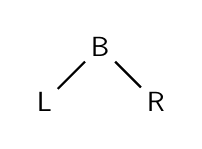
\begin{tikzpicture}
    \node (top) at (0,0) {$\mathsf{B}$};
    \node [below left  of=top] (left)  {$\mathsf{L}$};
    \node [below right of=top] (right) {$\mathsf{R}$};

    % Now draw the lines:
    \draw [thick, shorten <=-2pt, shorten >=-2pt] (top) -- (left);
    \draw [thick, shorten <=-2pt, shorten >=-2pt] (top) -- (right);
\end{tikzpicture}
\end{center}

What's interesting to note is that the points of $\mathsf{BCover}$ always have maxima with respect to specialization order. That means it's always possible to non-deterministically join points of $\mathsf{BCover}$ together.

Just as we found that the ``conjunction'' and ``disjunction'' operations of pairs of Coq propositions preserved having binary covers, we can define continuous maps representing conjunction and disjunction over the $\mathsf{BCover}$ space:
\begin{align*}
\cdot \wedge \cdot &: \mathsf{BCover} \times \mathsf{BCover} \to \mathsf{BCover}
\\ x \wedge y &\triangleq \mathsf{cases}(x, y)
\begin{cases}
\mathsf{Left}, \mathsf{Left}
 \quad &\Branch \quad
 \mathsf{L}
\\
\mathsf{Right}, \_\_
 \quad &\Branch \quad
 \mathsf{R}
\\
\_\_, \mathsf{Right}
 \quad &\Branch \quad
 \mathsf{R}
\end{cases}
\\
\cdot \vee \cdot &: \mathsf{BCover} \times \mathsf{BCover} \to \mathsf{BCover}
\\ x \vee y &\triangleq \mathsf{cases}(x, y)
\begin{cases}
\mathsf{Left}, \_\_
 \quad &\Branch \quad
 \mathsf{L}
\\
\_\_, \mathsf{Left}
 \quad &\Branch \quad
 \mathsf{L}
\\
 \mathsf{Right}, \mathsf{Right}
 \quad &\Branch \quad
 \mathsf{R}
\end{cases}.
\end{align*}

Are these definitions, using overlapping pattern matching, valid definitions? There are two conditions to check: that the cases cover the entire input space, and that overlapping branches have a maximum in terms of specialization order. Since the output space is $\mathsf{BCover}$, which always have maxima, we always satisfy the second condition. Since we have the cover
\[
\top_\mathsf{BCover} \le \mathsf{Left} \vee \mathsf{Right},
\]
we have in the product space
\begin{align*}
\top_{\mathsf{BCover} \times \mathsf{BCover}} \le 
  &(\mathsf{Left} \times \mathsf{Left}) \vee (\mathsf{Left} \times \mathsf{Right})
\\ \vee &(\mathsf{Right} \times \mathsf{Left}) \vee (\mathsf{Right} \times \mathsf{Right}),
\end{align*}
which clearly shows that the cases in the definitions of conjunction and disjunction also cover the entire input space.

It's still important to check that these definitions satisfy the definitions you'd expect for conjunction and disjunction on binary covers. Negation is easy as well:
\begin{align*}
 \neg &: \mathsf{BCover} \to \mathsf{BCover}
\\ \neg x &\triangleq \mathsf{cases}(x)
\begin{cases}
\mathsf{Left}
 \quad &\Branch \quad
 \mathsf{R}
\\
\mathsf{Right}
 \quad &\Branch \quad
 \mathsf{L}
\end{cases}
\end{align*}

\subsection{Alternative understandings of binary covers}

If you're bothered by the fact that the two opens in a binary cover get ``opposite'' treatments, and in particular that the logical operations on the second open are in reverse, for no good reason, there's another way to think about it. Rather than thinking of a binary cover of $A$ as two opens $P, Q : \Open{A}$ such that $A \subseteq P \cup Q$, we can instead think of it as an open set $P$ and a \emph{closed} set $\overline{Q}$ which is the ``set-theoretic'' complement of $Q$, since the complement of an open set is closed. Then the fact that $\langle P, Q \rangle$ is a binary cover means that $\overline{Q} \subseteq P$. Then the definitions of the logical operations should make more sense. For instance, one can find the union of two closed sets by taking their complement to produce two open sets, taking the intersection of that, and then taking the complement to return to a closed set. Since we are simply ``encoding'' closed sets with their open complements, computing the ``union'' just corresponds to taking an intersection.

This elicits the view of binary covers as ``approximate'' predicates, sandwiching a closed subspace inside an open one, with wiggle room for for points which are in between. Any points which are in $\overline{Q}$ (and thus also $P$) will definitely compute to $\mathsf{Left}$, while any points which are outside of $P$ (and thus also outside $\overline{Q}$) will definitely compute to $\mathsf{Right}$, while in-between points, which are in $P$ but not $\overline{Q}$, are allowed to compute either way.

Finally, note that there is a homeomorphism $\mathsf{BCover} \cong \PLower^+(\bool)$ given by
\begin{align*}
\mathsf{to} &: \mathsf{BCover} \to \PLower^+(\bool)
\\ \mathsf{to}(x) &\triangleq
  \mathsf{cases}(x)
  \begin{cases}
\mathsf{Left}
 \quad &\Branch \quad
 \{ \mathsf{tt} \}
\\
\mathsf{Right}
 \quad &\Branch \quad
 \{ \mathsf{ff} \}
  \end{cases}
\\
\mathsf{from} &: \PLower^+(\bool) \to \mathsf{BCover}
\\ \mathsf{from}(s) &\triangleq
  \mathsf{cases}(s)
  \begin{cases}
 \oincl{\lozenge(\cdot = \mathsf{tt})}{\wildcard}
 \quad &\Branch \quad
 \mathsf{L}
\\
 \oincl{\lozenge(\cdot = \mathsf{ff})}{\wildcard}
 \quad &\Branch \quad
 \mathsf{R}
  \end{cases},
\end{align*}
which gives another understanding of binary covers, as representing non-deterministic truth values in Boolean logic. All of the logical operations defined for binary covers might make more sense when interpreted by the homeomorphism above. For instance, the conjunction operation on Boolean values,
$\&\& : \bool \times \bool \to \bool$ can be lifted to a function of type $\PLower(\bool) \times \PLower(\bool) \to \PLower(\bool)$ which applies $\&\&$ to its non-deterministic input possibilities and collects all the possible results. This lifted $\&\&$ operation, when translated by the above homeomorphism to $\mathsf{BCover}$, identical to the $\wedge$ operation on $\mathsf{BCover}$s. This applies similarly to the other logical connectives that were defined on $\mathsf{BCover}$s.

This allows us to easily confirm that the logical connectives that we defined for $\mathsf{BCover}$s satisfy  De Morgan's laws for Boolean logic. In fact, binary covers form what is called a quasi-Boolean algebra, which satisfy almost all of the laws of Boolean algebra. Binary covers are similar to the three-valued logic K3, and also related to 

The specialization order on $\mathsf{BCover}$s corresponds to subset inclusion on $\PLower(\bool)$.

\section{Related work}

\cite{coquand1992} gives a topologically motivated explanation of pattern matching for dependently typed functional programming, describing patterns as (disjoint) partitions of a space.

\cite{dijkstra} introduces ``guarded commands'', a language construct for imperative programming languages, where a branch can be chosen from a list of statements each guarded by boolean expressions. Whereas the cases in \cite{dijkstra} must be each decidable, in this work this need not be the case.

Vickers?

dReal is a tool which allows computation of approximate truth values over the real numbers \cite{dReal}, allowing order comparisons and bounded quantifiers. The calculus of binary covers presented here, when restricted to $\R$, provides similar computational abilities, but with a different foundational framework. In a sense, it shows how it is possible to generalize the theory behind dReal to general topological spaces.

\section{Conclusion}
Isn't life great?

Future work:
\begin{itemize}
\item Extend to the gros topos, higher order functions, Kan extensions, that kind of thing
\item Find other toposes, perhaps, which have notions of non-determinism or something like a specialization order, which would allow overlapping patterns to be meaningful
\end{itemize}


% conference papers do not normally have an appendix


% use section* for acknowledgment
\section*{Acknowledgment}


The authors would like to thank...





% trigger a \newpage just before the given reference
% number - used to balance the columns on the last page
% adjust value as needed - may need to be readjusted if
% the document is modified later
%\IEEEtriggeratref{8}
% The "triggered" command can be changed if desired:
%\IEEEtriggercmd{\enlargethispage{-5in}}

% references section

% can use a bibliography generated by BibTeX as a .bbl file
% BibTeX documentation can be easily obtained at:
% http://mirror.ctan.org/biblio/bibtex/contrib/doc/
% The IEEEtran BibTeX style support page is at:
% http://www.michaelshell.org/tex/ieeetran/bibtex/
%\bibliographystyle{IEEEtran}
% argument is your BibTeX string definitions and bibliography database(s)
%\bibliography{IEEEabrv,../bib/paper}
%
% <OR> manually copy in the resultant .bbl file
% set second argument of \begin to the number of references
% (used to reserve space for the reference number labels box)
\bibliographystyle{IEEEtran}
\bibliography{LICS}




% that's all folks
\end{document}


